\documentclass{standalone}
\usepackage{tikz}
\usetikzlibrary{patterns, positioning}
\usepackage[sfdefault]{ClearSans} %% option 'sfdefault' activates Clear Sans as the default text font
\usepackage[T1]{fontenc}

\begin{document}
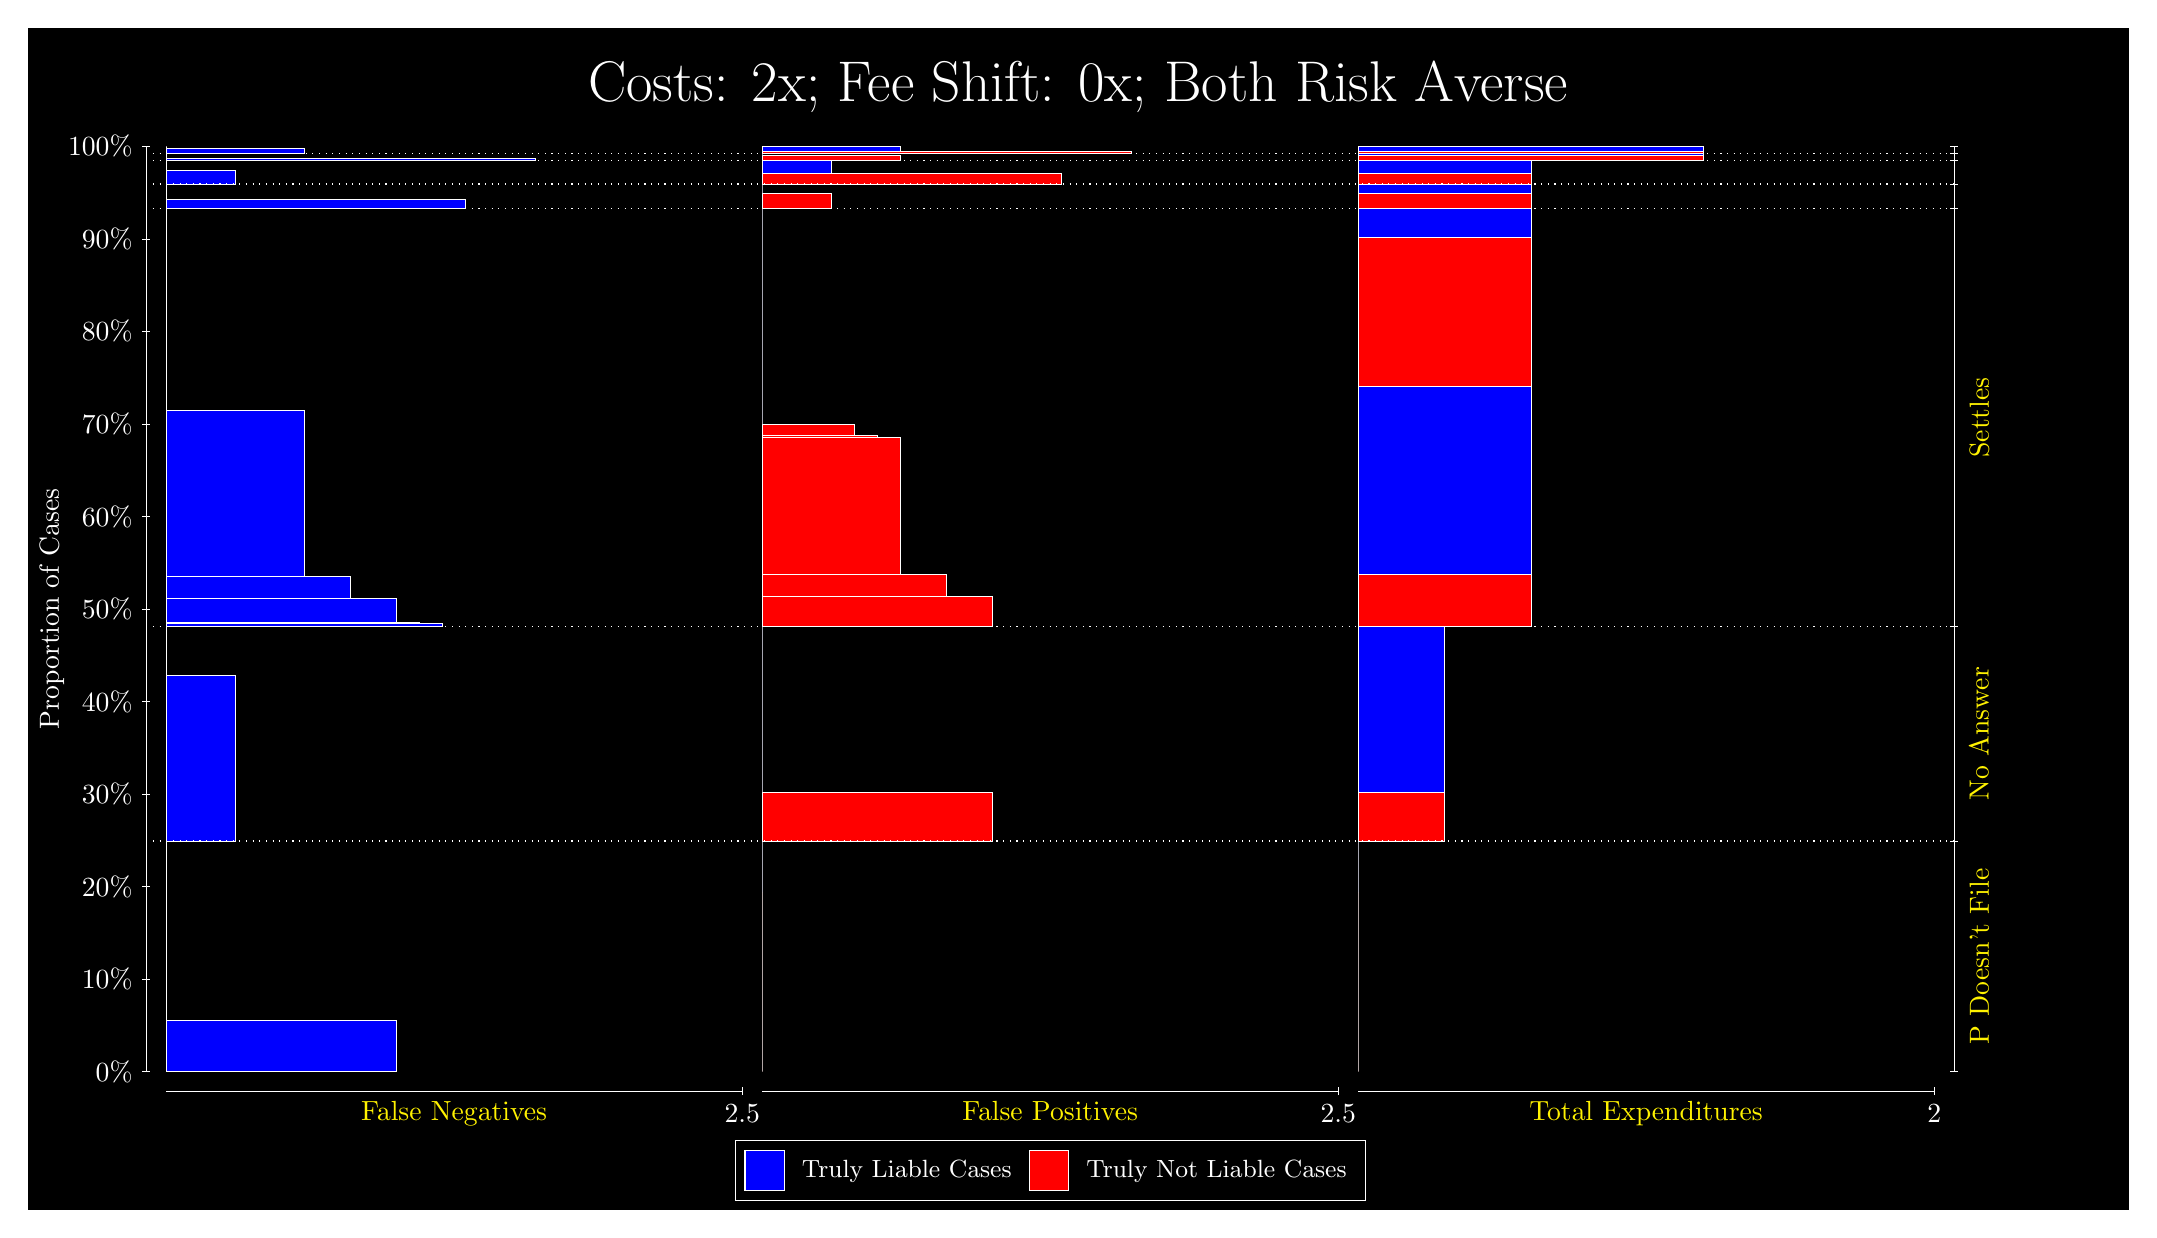
\begin{tikzpicture}
\draw[fill=black] (0,0) rectangle (26.667,15);
\draw[text=white] (0,13.5) rectangle (26.667,15) node[midway] {\huge Costs: 2x; Fee Shift: 0x; Both Risk Averse};
\draw[white, very thin] (1.5,1.75) -- (1.5,13.5);
\node[rotate=90, text=white, anchor=center] at (0.3, 7.625) {Proportion of Cases};
\draw[white, very thin] (1.45,1.75) -- (1.55,1.75);
\node[text=white, anchor=east] at (1.45, 1.75) {0\%};
\draw[white, very thin] (1.45,2.925) -- (1.55,2.925);
\node[text=white, anchor=east] at (1.45, 2.925) {10\%};
\draw[white, very thin] (1.45,4.1) -- (1.55,4.1);
\node[text=white, anchor=east] at (1.45, 4.1) {20\%};
\draw[white, very thin] (1.45,5.275) -- (1.55,5.275);
\node[text=white, anchor=east] at (1.45, 5.275) {30\%};
\draw[white, very thin] (1.45,6.45) -- (1.55,6.45);
\node[text=white, anchor=east] at (1.45, 6.45) {40\%};
\draw[white, very thin] (1.45,7.625) -- (1.55,7.625);
\node[text=white, anchor=east] at (1.45, 7.625) {50\%};
\draw[white, very thin] (1.45,8.8) -- (1.55,8.8);
\node[text=white, anchor=east] at (1.45, 8.8) {60\%};
\draw[white, very thin] (1.45,9.975) -- (1.55,9.975);
\node[text=white, anchor=east] at (1.45, 9.975) {70\%};
\draw[white, very thin] (1.45,11.15) -- (1.55,11.15);
\node[text=white, anchor=east] at (1.45, 11.15) {80\%};
\draw[white, very thin] (1.45,12.325) -- (1.55,12.325);
\node[text=white, anchor=east] at (1.45, 12.325) {90\%};
\draw[white, very thin] (1.45,13.5) -- (1.55,13.5);
\node[text=white, anchor=east] at (1.45, 13.5) {100\%};

\draw[white, very thin] (24.457,1.75) -- (24.457,13.5);
\draw[white, very thin] (24.407,1.75) -- (24.507,1.75);
\node[anchor=west] at (24.407, 1.75) {};
\draw[white, very thin] (24.407,4.6772) -- (24.507,4.6772);
\node[anchor=west] at (24.407, 4.6772) {};
\draw[white, very thin] (24.407,7.4024) -- (24.507,7.4024);
\node[anchor=west] at (24.407, 7.4024) {};
\draw[white, very thin] (24.407,12.709) -- (24.507,12.709);
\node[anchor=west] at (24.407, 12.709) {};
\draw[white, very thin] (24.407,13.022) -- (24.507,13.022);
\node[anchor=west] at (24.407, 13.022) {};
\draw[white, very thin] (24.407,13.322) -- (24.507,13.322);
\node[anchor=west] at (24.407, 13.322) {};
\draw[white, very thin] (24.407,13.413) -- (24.507,13.413);
\node[anchor=west] at (24.407, 13.413) {};
\draw[white, very thin] (24.407,13.5) -- (24.507,13.5);
\node[anchor=west] at (24.407, 13.5) {};

\draw[white, very thin, fill=blue] (1.75,1.75) rectangle (4.6775,2.3982);
\draw[white, very thin, fill=red] (1.75,2.3982) rectangle (1.75,4.6772);
\draw[white, very thin, fill=blue] (1.75,4.6772) rectangle (2.6283,6.7825);
\draw[white, very thin, fill=red] (1.75,6.7825) rectangle (1.75,7.4024);
\draw[white, very thin, fill=blue] (1.75,7.4024) rectangle (5.2631,7.4431);
\draw[white, very thin, fill=blue] (1.75,7.4431) rectangle (4.9703,7.453);
\draw[white, very thin, fill=blue] (1.75,7.453) rectangle (4.6775,7.7646);
\draw[white, very thin, fill=blue] (1.75,7.7646) rectangle (4.092,8.0388);
\draw[white, very thin, fill=blue] (1.75,8.0388) rectangle (3.5065,10.143);
\draw[white, very thin, fill=red] (1.75,10.143) rectangle (1.75,12.709);
\draw[white, very thin, fill=blue] (1.75,12.709) rectangle (5.5558,12.833);
\draw[white, very thin, fill=red] (1.75,12.833) rectangle (1.75,13.022);
\draw[white, very thin, fill=blue] (1.75,13.022) rectangle (2.6283,13.193);
\draw[white, very thin, fill=red] (1.75,13.193) rectangle (1.75,13.322);
\draw[white, very thin, fill=blue] (1.75,13.322) rectangle (6.4341,13.35);
\draw[white, very thin, fill=red] (1.75,13.35) rectangle (1.75,13.413);
\draw[white, very thin, fill=blue] (1.75,13.413) rectangle (3.5065,13.472);
\draw[white, very thin, fill=red] (1.75,13.472) rectangle (1.75,13.5);
\draw[white, very thin, fill=red] (9.3189,1.75) rectangle (9.3189,4.029);
\draw[white, very thin, fill=blue] (9.3189,4.029) rectangle (9.3189,4.6772);
\draw[white, very thin, fill=red] (9.3189,4.6772) rectangle (12.246,5.2971);
\draw[white, very thin, fill=blue] (9.3189,5.2971) rectangle (9.3189,7.4024);
\draw[white, very thin, fill=red] (9.3189,7.4024) rectangle (12.246,7.7906);
\draw[white, very thin, fill=red] (9.3189,7.7906) rectangle (11.661,8.0698);
\draw[white, very thin, fill=red] (9.3189,8.0698) rectangle (11.075,9.7996);
\draw[white, very thin, fill=red] (9.3189,9.7996) rectangle (10.783,9.8283);
\draw[white, very thin, fill=red] (9.3189,9.8283) rectangle (10.49,9.9689);
\draw[white, very thin, fill=blue] (9.3189,9.9689) rectangle (9.3189,12.709);
\draw[white, very thin, fill=red] (9.3189,12.709) rectangle (10.197,12.899);
\draw[white, very thin, fill=blue] (9.3189,12.899) rectangle (9.3189,13.022);
\draw[white, very thin, fill=red] (9.3189,13.022) rectangle (13.125,13.152);
\draw[white, very thin, fill=blue] (9.3189,13.152) rectangle (10.197,13.322);
\draw[white, very thin, fill=red] (9.3189,13.322) rectangle (11.075,13.386);
\draw[white, very thin, fill=blue] (9.3189,13.386) rectangle (9.3189,13.413);
\draw[white, very thin, fill=red] (9.3189,13.413) rectangle (14.003,13.441);
\draw[white, very thin, fill=blue] (9.3189,13.441) rectangle (11.075,13.5);
\draw[white, very thin, fill=red] (16.888,1.75) rectangle (16.888,4.029);
\draw[white, very thin, fill=blue] (16.888,4.029) rectangle (16.888,4.6772);
\draw[white, very thin, fill=red] (16.888,4.6772) rectangle (17.986,5.2971);
\draw[white, very thin, fill=blue] (16.888,5.2971) rectangle (17.986,7.4024);
\draw[white, very thin, fill=red] (16.888,7.4024) rectangle (19.083,8.0698);
\draw[white, very thin, fill=blue] (16.888,8.0698) rectangle (19.083,10.448);
\draw[white, very thin, fill=red] (16.888,10.448) rectangle (19.083,12.347);
\draw[white, very thin, fill=blue] (16.888,12.347) rectangle (19.083,12.709);
\draw[white, very thin, fill=red] (16.888,12.709) rectangle (19.083,12.899);
\draw[white, very thin, fill=blue] (16.888,12.899) rectangle (19.083,13.022);
\draw[white, very thin, fill=red] (16.888,13.022) rectangle (19.083,13.152);
\draw[white, very thin, fill=blue] (16.888,13.152) rectangle (19.083,13.322);
\draw[white, very thin, fill=red] (16.888,13.322) rectangle (21.279,13.386);
\draw[white, very thin, fill=blue] (16.888,13.386) rectangle (21.279,13.413);
\draw[white, very thin, fill=red] (16.888,13.413) rectangle (21.279,13.441);
\draw[white, very thin, fill=blue] (16.888,13.441) rectangle (21.279,13.5);
\draw[white, dotted] (1.5,4.6772) -- (24.457,4.6772);
\draw[white, dotted] (1.5,7.4024) -- (24.457,7.4024);
\draw[white, dotted] (1.5,12.709) -- (24.457,12.709);
\draw[white, dotted] (1.5,13.022) -- (24.457,13.022);
\draw[white, dotted] (1.5,13.322) -- (24.457,13.322);
\draw[white, dotted] (1.5,13.413) -- (24.457,13.413);
\draw[white, very thin] (1.75,1.5) -- (9.0689,1.5);
\node[text=yellow, anchor=north] at (5.4094, 1.5) {False Negatives};
\draw[white, very thin] (9.0689,1.45) -- (9.0689,1.55);
\node[text=white, anchor=north] at (9.0689, 1.45) {2.5};

\draw[white, very thin] (9.3189,1.5) -- (16.638,1.5);
\node[text=yellow, anchor=north] at (12.978, 1.5) {False Positives};
\draw[white, very thin] (16.638,1.45) -- (16.638,1.55);
\node[text=white, anchor=north] at (16.638, 1.45) {2.5};

\draw[white, very thin] (16.888,1.5) -- (24.207,1.5);
\node[text=yellow, anchor=north] at (20.547, 1.5) {Total Expenditures};
\draw[white, very thin] (24.207,1.45) -- (24.207,1.55);
\node[text=white, anchor=north] at (24.207, 1.45) {2};

\node[text=yellow, centered, rotate=90] at (24.777, 3.2136) {P Doesn't File};
\node[text=yellow, centered, rotate=90] at (24.777, 6.0398) {No Answer};
\node[text=yellow, centered, rotate=90] at (24.777, 10.056) {Settles};





\draw (12.978300999999998,1.5) node[draw=none] (baseCoordinate) {};
\begin{scope}[align=center]
        \matrix[scale=0.5, draw=white, below=0.5cm of baseCoordinate, nodes={draw}, column sep=0.1cm]{
            \node[rectangle, draw, minimum width=0.5cm, minimum height=0.5cm, fill=blue] {}; &
            \node[draw=none, font=\small, text=white] (B) {Truly Liable Cases}; &
            \node[rectangle, draw, minimum width=0.5cm, minimum height=0.5cm, fill=red] {}; &
            \node[draw=none, font=\small, text=white] (B) {Truly Not Liable Cases}; \\
            };
\end{scope}

\end{tikzpicture}
\end{document}